\begin{figure}[htbp]
\vspace{-10pt}
        \centering
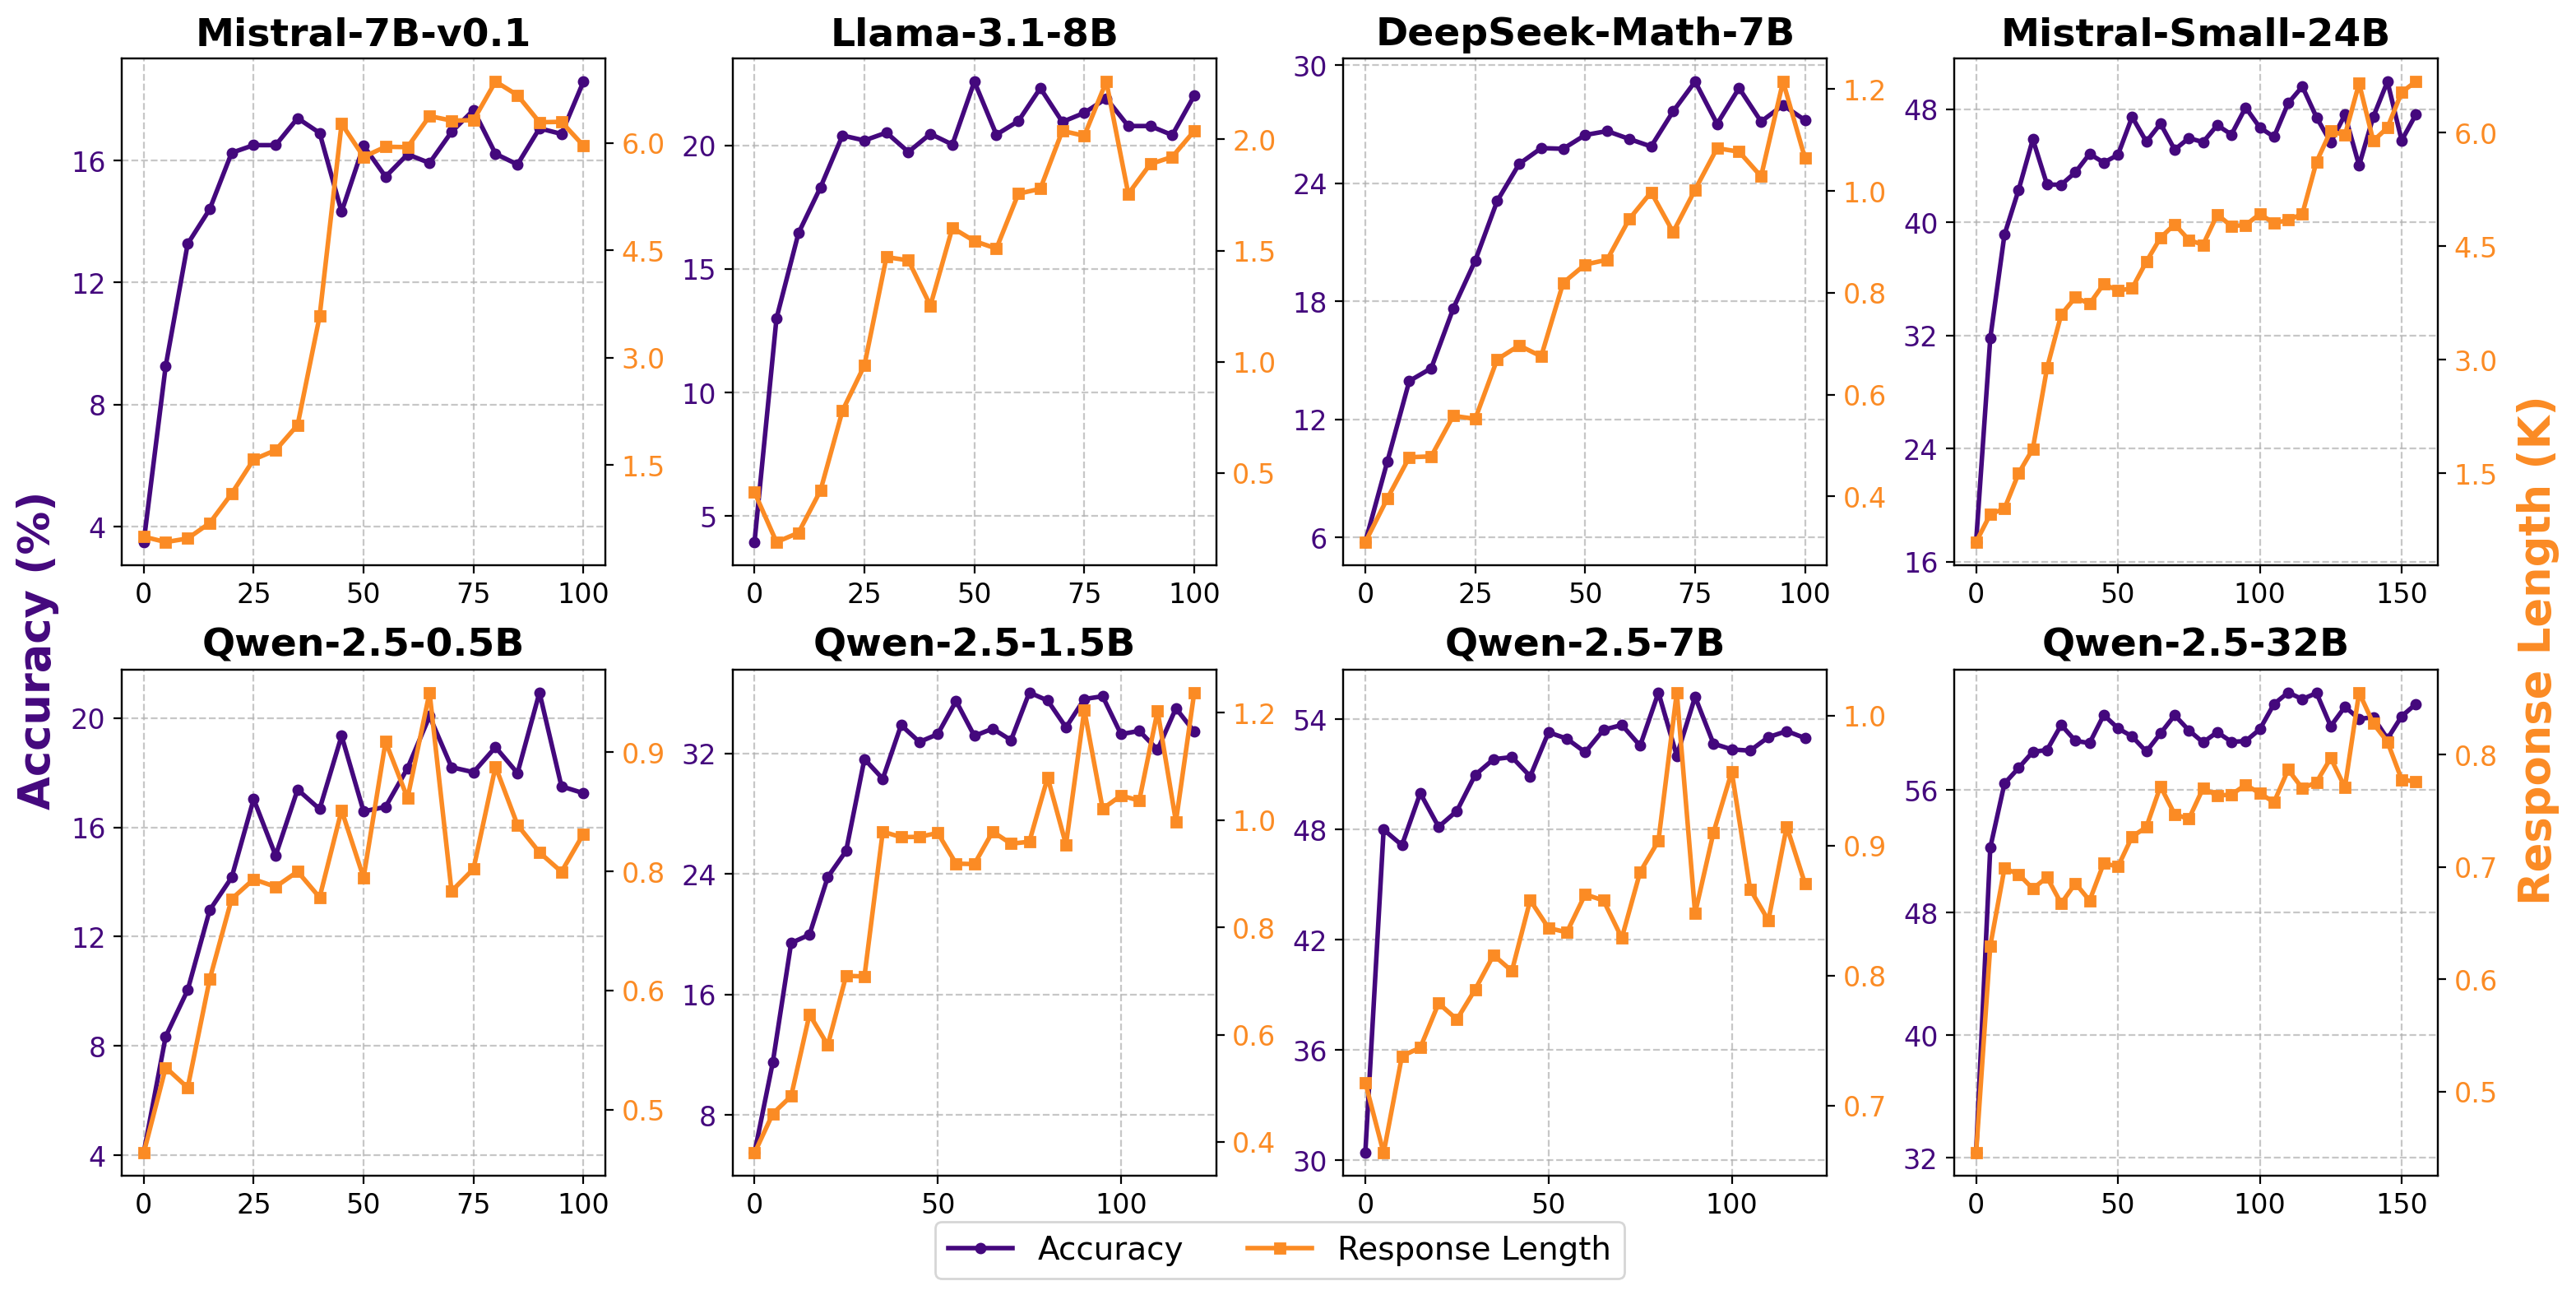
\includegraphics[width=0.98\textwidth]{fig/plot_figure1_v2.3_token_length_vs_steps.pdf}
\vspace{-10pt}
\caption{Accuracy and response length across training iterations for different models, averaged on GSM8K, MATH500, Minerva Math, OlympiadBench, AIME24, and AMC23. Per-benchmark results are in Figure~\ref{fig:appx_acc&len} (Appendix~\ref{appx:DetailedResult}). All training starts from base models.
% All models are trained starting from their base version.
        }
        \label{fig1:acc&len}
    \vspace{-10pt}
\end{figure}


\section{Introduction}
Large reasoning models, including OpenAI-o1~\citep{jaech2024openai}, DeepSeek-R1~\citep{guo2025deepseek}, and Kimi-k1.5~\citep{team2025kimi}, demonstrate remarkable abilities. These models excel at generating long Chains-of-Thought (CoT)~\citep{wei2022chain} responses when solving complex tasks and exhibit advanced, reflection-like reasoning behaviors. 
Recently, DeepSeek-R1~\citep{guo2025deepseek} has revealed that starting from pretrained models (i.e., base models), pure reinforcement learning (RL) with rule-based reward can lead to the spontaneous emergence of long CoT and self-reflection behaviors, called the ``aha moment''. This RL training paradigm starting from base models is often referred to as \emph{zero RL training}.

% Despite DeepSeek's generous open-sourcing of their models, the community still lacks a sufficient understanding of the "zero training" process. 
While the success of zero RL training was initially demonstrated using DeepSeek-V3~\citep{deepseekai2025deepseekv3technicalreport}, a model with 671B parameters, it remained unclear whether such emergent phenomena persist in generally smaller and less capable open base models.
Recent open-source efforts exploring zero-training approaches have predominantly centered on the Qwen2.5-series models~\citep{zeng2025simplerl,yeo2025demystifying,xie2025logic,OpenReasonerZero2025,yu2025dapoopensourcellmreinforcement}, which, even as base models, exhibit strong instruction-following capabilities and display notable cognitive behaviors such as backtracking and verification from the beginning, as we will detail in \S\ref{sec:qwen_behabiur}.
Moreover, the analyses of model behavior in these studies remain largely superficial, focusing primarily on metrics such as response length and accuracy. These observations neither clearly establish whether the models' reasoning behaviors actually change nor clarify the mechanisms underlying the emergence of effective reasoning, leaving a significant gap in understanding.
% Although DeepSeek has generously open-sourced their models, the research community still lacks a deep understanding of the ``zero training" mechanism. Most existing analyses remain superficial—primarily noting increased response lengths or shifts in word frequency—without clearly linking these observations to the underlying mechanisms that enable effective reasoning behaviors to emerge~\citep{OpenReasonerZero2025,yeo2025demystifying,xie2025logic}.

To provide a more transparent understanding of zero RL training across different base models in the wild, this paper addresses the following key questions: (1) How do reasoning capabilities develop across various models during zero RL training? (2) Does an ``aha moment'' still occur for base models that initially lack strong instruction-following and self-verification abilities? (3) What are the critical factors for ensuring successful zero RL training across diverse base models?

% Why did previous attempts at ``zero-training" typically fail for most base models? What are the key secrets that enable successful ``zero-training" of these models?
%(3) How does the difficulty of emergent reflection behavior vary with different base models? 

%(3) Do traditional supervised fine-tuning (SFT) methods—such as enforcing shorter CoT~\citep{yu2023metamath,luo2023wizardmath}—impede the natural development of complex reasoning patterns?

To this end, we perform zero RL training across a diverse range of model series and sizes, including Mistral-7B~\citep{jiang2023mistral7b}, Mistral-24B~\citep{mistral2024small}, Llama3-8B~\citep{dubey2024llama}, DeepSeek-Math-7B~\citep{shao2024deepseekmath}, Qwen2.5-0.5B/1.5B/7B/14B/32B~\citep{yang2024qwen2}, as well as Qwen2.5-Math-7B~\citep{yang2024qwen2math}. 
% To keep the recipe simple, our experiments rely solely on the GSM8K~\citep{cobbe2021training} and MATH~\citep{hendrycks2021measuring} training data, for rule-based reward modeling. 
To maintain simplicity in the training recipe, our experiments rely exclusively on the training sets of GSM8K~\citep{cobbe2021training} and MATH~\citep{hendrycks2021measuring} datasets for rule-based reward modeling.
It is worth noting that we adopt the same training hyperparameters to train all the models.
Using GRPO~\citep{shao2024deepseekmath} as the RL algorithm, combined with several critical factors that we identified, we obtain significant improvements in model accuracy across all base models, along with a notable increase in response length for 9 out of the 10 models, with the exception of Qwen2.5-Math-7B. 
However, through careful monitoring of training dynamics and reasoning behaviors, we find that different base models exhibit distinct patterns during training. Also, certain specific factors require careful attention to ensure successful zero RL training. Below, we summarize our key findings.
\begin{tcolorbox}[colback=lightblue!80,breakable]
\begin{enumerate}[leftmargin=1em]
    \item Increased response length does not always correspond to an ``aha moment'' -- Interestingly, for most Qwen2.5 models, which form the foundation of most recent open-source efforts, we do not observe a rise in the frequency of certain cognitive behaviors, such as self-reflection, despite the increase in response length. (\textsection\ref{sec:qwen_behabiur})
    \item For the first time, we observe a significant increase in the frequency of specific cognitive reasoning behaviors, such as verification, in small models outside the Qwen family, notably in the Llama3-8B and DeepSeek-Math-7B models. (\textsection\ref{sec:deepseek-math_behabiur})
    % \qian{And we may highlight the contribution of using the same hyper-parameter on all models to make their response length increasing and performance increasing?}
    % \qian{For the first time, we observe a significant increase in the frequency of specific cognitive reasoning behaviors, such as verification, in small models not from Qwen family, the Llama3-8B and DeepSeek-Math-7B models.}
    \item Enforcing rigid format reward (e.g., enclosing answers within boxes)~\citep{guo2025deepseek} significantly penalizes exploration~\citep{singh2023beyond,wang2024planning}, particularly for base models that initially struggle with instruction following. This restriction lowers their  performance ceiling and often induces overthinking behaviors~\citep{chen2024not}. (\textsection\ref{sec:remove_format})
    \item The difficulty level of the training data must align closely with the base model's intrinsic exploration capabilities, otherwise zero RL will fail. (\textsection\ref{sec:data_complextiy_behaviur})
    \item In contrast to the observation in~\citet{shao2024deepseekmath}, zero RL training lifts pass@k accuracy by 10-30 absolute points, a strong evidence confirming zero RL training is not just reranking responses. (\textsection\ref{sec:lift_pass_k})
    \item We revisit the traditional training pipeline that performs SFT to learn to follow instructions before RL training. Specifically, we use conventional SFT datasets as a cold start for RL—a de facto approach prior to the release of DeepSeek-R1. While high-quality CoT data~\citep{li2024numinamath} can rapidly enhance a base model's performance through imitation, we find that it significantly limits the model's ability to explore freely during RL. This constraint diminishes post-RL performance and suppresses the emergence of advanced reasoning capabilities. (\textsection\ref{sec:short_cot_influence})
\end{enumerate}
\end{tcolorbox}

% The results reveal substantial performance improvements and notable increases in CoT length across all tested models. Additionally, we perform comprehensive, real-time monitoring of CoT dynamics and reasoning behavior throughout the training process. Notably, we observe the emergence of reflection patterns from scratch, consistently appearing across different models.

% In our experiments, we identify several critical challenges that impact the stability and performance limits of ``zero training" and devise targeted solutions to mitigate them. 
%(1) We observe that weak zero-shot capabilities ~\citep{wei2021finetuned} in most base models lead to excessively long, irrelevant responses, causing training instability. 
%To mitigate this, we customize prompt templates ~\citep{yang2024qwen2} per model and apply precise truncation with carefully chosen stop tokens during rollout. (this part can in our analyse)
% (1) We observe that enforcing rigid formatting constraints (e.g., enclosing answers within boxes)~\citep{guo2025deepseek} significantly limits exploration~\citep{singh2023beyond,wang2024planning}, particularly in weaker models. This restriction lowers their potential performance ceiling and often induces overthinking behaviors~\citep{chen2024not}. 
%Consequently, we remove format-based rewards in our formal experiments, allowing models to explore freely. This adjustment leads to steadier improvements in reasoning efficiency and ultimately results in higher peak performance. 
% (22) We also observe that the difficulty level of the training data must align closely with the base model's intrinsic exploration capabilities. 
%Data that is too challenging or overly simplistic can impede effective exploration and hinder training progress, a result consistent with findings in prior research~\citep{cui2025process,team2025kimi}. 
% (3) Additionally, we observe that specific exploration-related hyperparameters, particularly sampling size and temperature, can also influence the effectiveness of "zero training".
% (4) We re-evaluate the impact of traditional SFT methods on model exploration and uncover a surprising limitation: while high-quality short CoT data~\citep{li2024numinamath} can quickly enhance a base model's performance through imitation, it significantly constrains the model's ability to explore freely during RL. This restriction imposes a performance ceiling and stifles the emergence of advanced reasoning capabilities. 

%Our findings highlight the need for future cold-start strategies to prioritize exploration capacity—whether by incorporating long CoT data~\citep{guo2025deepseek,yeo2025demystifying} or designing SFT techniques~\citep{li2025preserving} that strike a balance between imitation and exploration—to enable sustained improvements in model reasoning performance.

% TODO: discuss the emergence phenomena on different base models

% TODO: dsicuss the impact of SFT to RL


% \begin{figure}[!t]
%         \centering
% 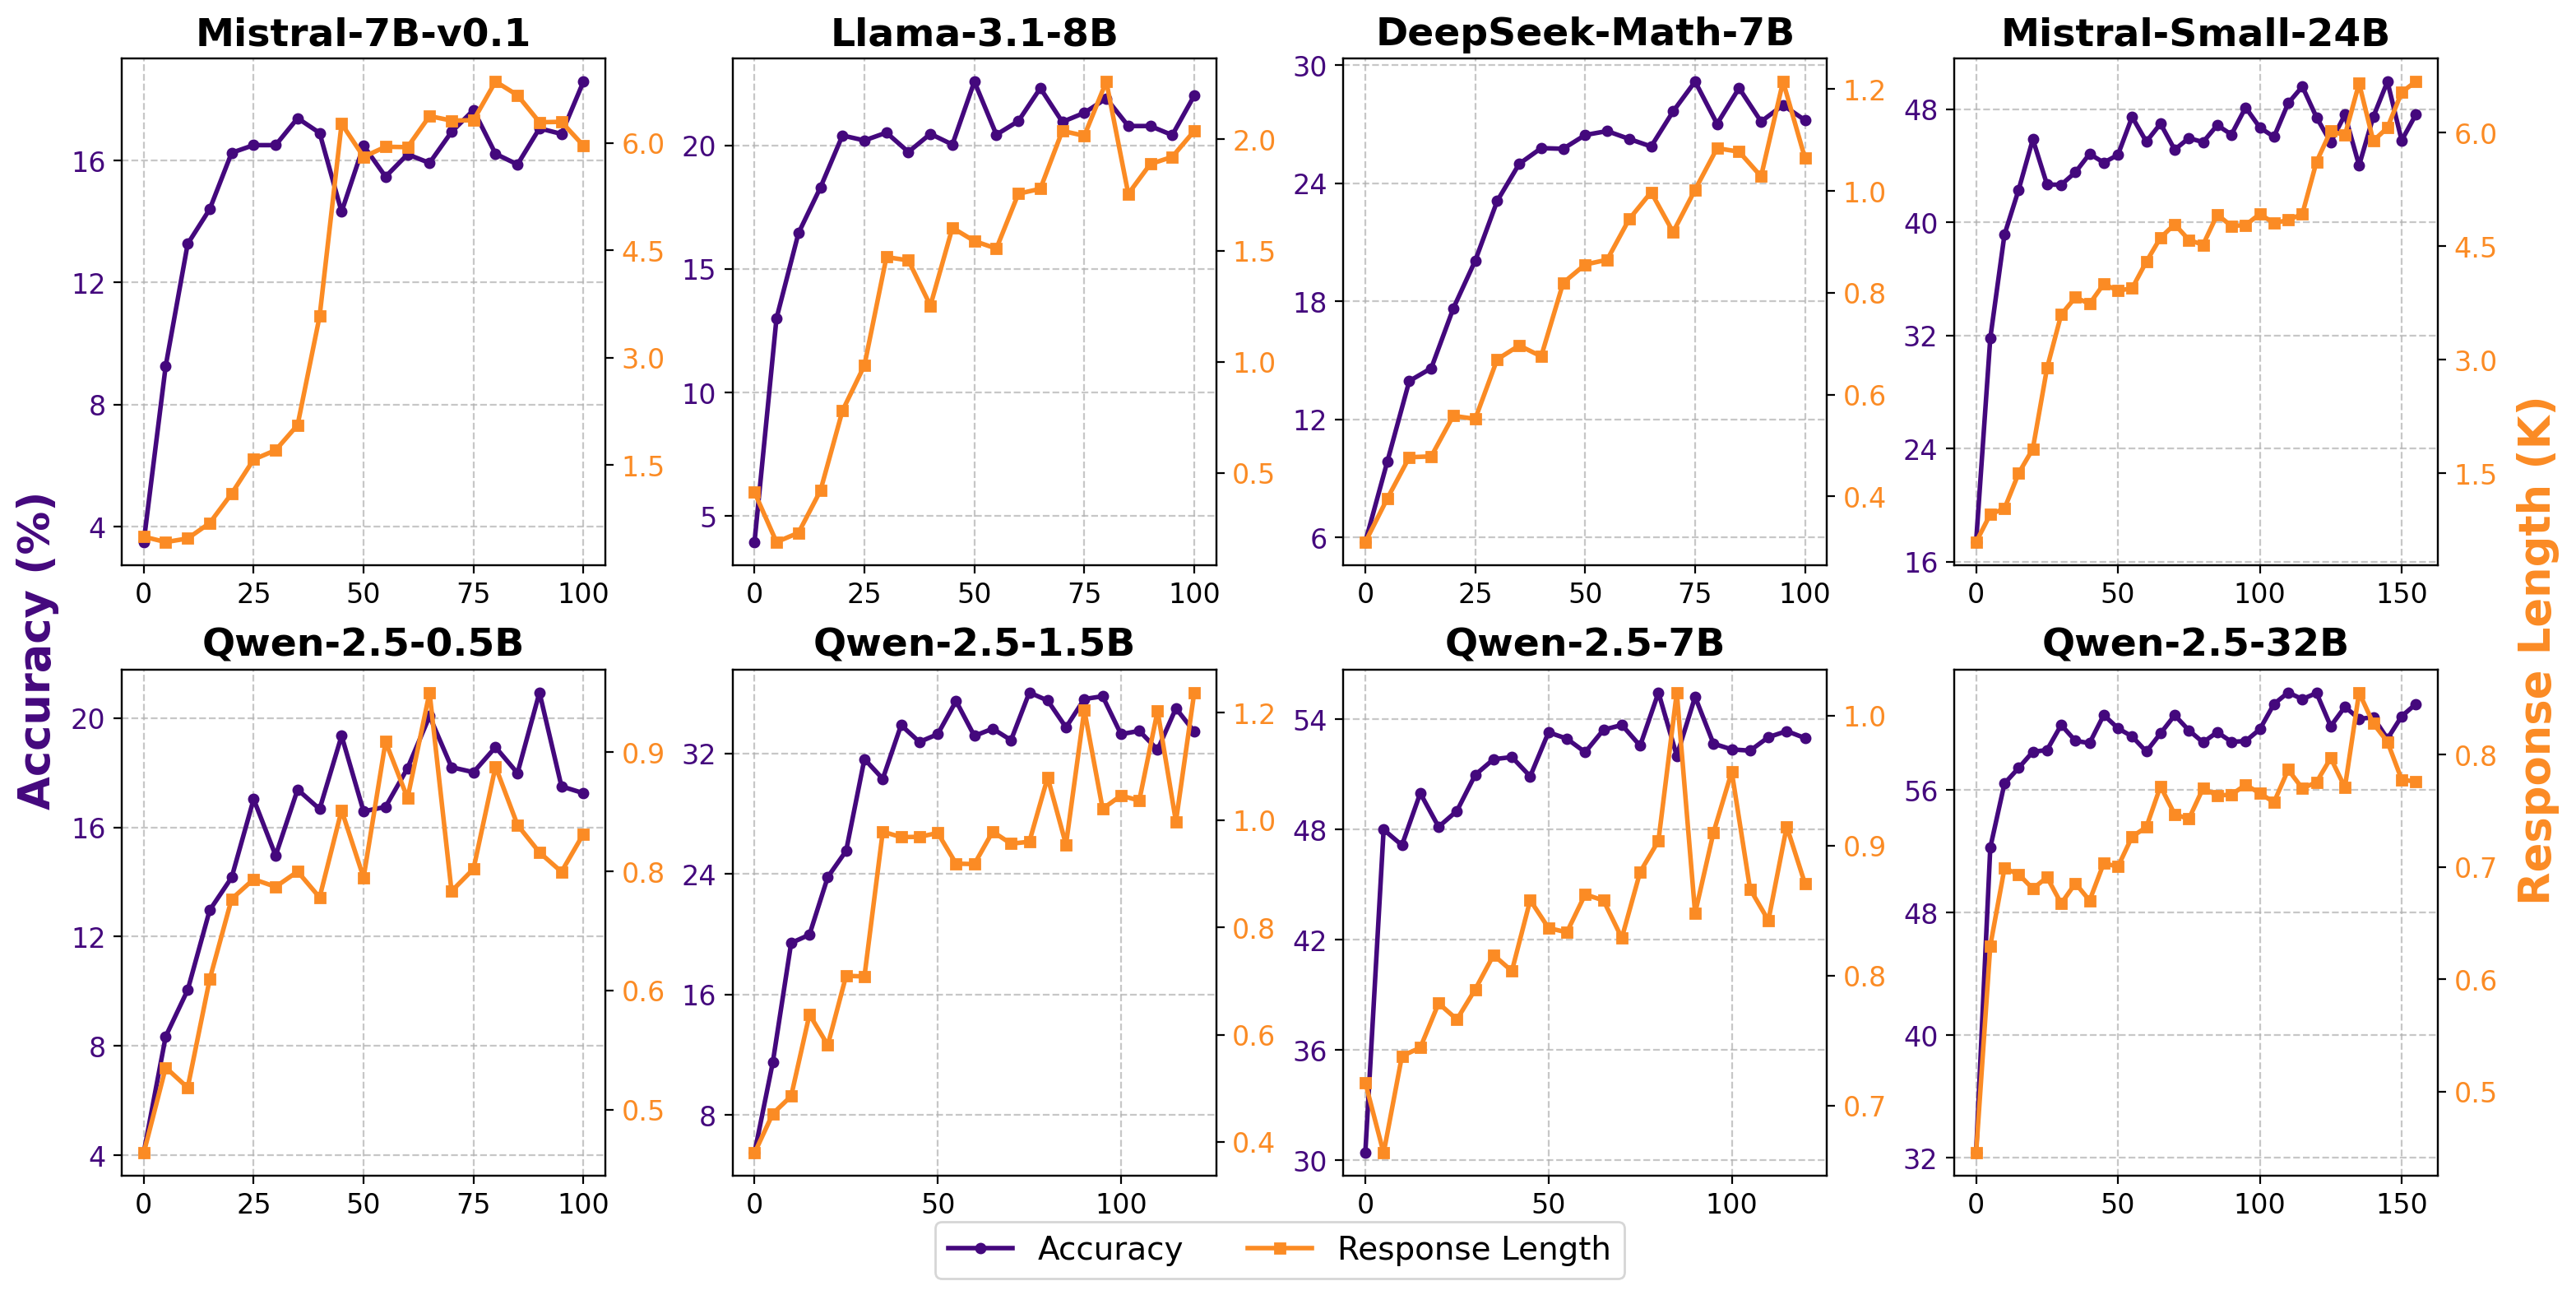
\includegraphics[width=\columnwidth]{fig/plot_figure1_v2.3_token_length_vs_steps.pdf}
% \caption{Average evaluation accuracy and response length across training steps for different models. We assess the models every five steps on a variety of math benchmarks, including GSM8K, MATH500, Minerva Math, and OlympiadBench, as well as competition-level benchmarks like AIME24 and AMC23. The purple line indicates the accuracy trend, while the yellow line represents the response length.
%         }
%         \label{fig1:acc&len}
%     \vspace{-10pt}
% \end{figure}